\documentclass[french,a4paper]{article}

\usepackage[utf8]{inputenc}          % Encodage des entrées
\usepackage[T1]{fontenc}             % Encodage de la fonte
\usepackage{babel}                   % Paquet de langue pour le français
\usepackage[margin=2.5cm]{geometry}  % Définition des marges
\usepackage{enumitem}                % Modification esthétique des listes
\usepackage{graphicx}   	         % Images

\PassOptionsToPackage{hyphens}{url}  % Les URL peuvent être écrits sur plusieurs lignes
\usepackage{hyperref}                % Les URL sont cliquables

\setlength{\parindent}{2em}          % Espace horizontal au début des paragraphes
\setlength{\parskip}{0.5em}          % Espace vertical entre les paragraphes
\renewcommand{\baselinestretch}{1.1} % Espace vertical entre les lignes

\title{La Première Guerre mondiale à travers les tensions entre les Suisses romands et alémaniques}
\author{\bsc{Beuchat} Bastien \and \bsc{Ding} Markus \and \bsc{Jollès} Eric \and \bsc{Mamie} Robin}
\date{24 avril 2020} % Date du rendu intermédiaire avec méthodologies et interprétations
%\date{13 mai 2020} % Date du rendu final

\begin{document}

\maketitle

% TODO
% - Faire la différence entre presse romande et Romands (resp. presse alémanique et Suisses allemands) (notamment dans le titre)
% - Mettre que du présent pour rapport final (pas de futur dans la méthodologie)
% - Inclure la frise chronologique utilisée dans la présentation
% - Ne pas exclure de devoir parler d'aspects économiques (ex: grève générale a un fort contexte économique, échanges commerciaux avec certains pays, ...)
% - Se concentrer sur l'analyse qualitative de la NZZ, et ne pas forcément faire de comparaison, mais se servir de cette analyse pour appuyer (éclairer) nos propos du côté romand (?)
% - Parler du manque d'articles du JDG entre 1917 et 1919 compris (ils n'existent pas)

\section*{Introduction}

\subsection*{Contexte historique}

En 1914, l’Europe est sous haute tension.
L’assassinat à Sarajevo de l'héritier du trône austro-hongrois, l'archiduc François-Ferdinand, est l’étincelle qui déclenche la Première Guerre mondiale. 
La Suisse se retrouve alors au centre du conflit, encerclée de toutes parts par les nations belligérantes qui constituent la Triple-Entente (France, Royaume-Uni, Russie) et la Triple-Alliance (Allemagne, Autriche-Hongrie, Italie).

La Suisse romande et la Suisse alémanique, de part leurs proximités culturelles et linguistiques avec les belligérants, ont différentes visions du conflit \cite{division}; l'unité du pays semble compromise.
L'élection du général de l'armée suisse Ulrich Wille \cite{wahl} va mettre à mal celle-ci. 
En effet plusieurs aspects le desservent: né à Hambourg, il est d'origine allemande et parle le Hochdeutsch à la place d'un dialecte suisse allemand.
La presse romande dénonce sa proximité culturelle, politique et militaire avec l'Allemagne pendant la guerre; il proposa par exemple d'entrer en guerre aux côtés des Empires centraux \cite{krieg}.

La plupart des journaux des deux régions linguistiques attisent alors les tensions en reprenant la propagande française ou allemande \cite{place} \cite{propagande} comme par exemple pour l'invasion de la Belgique par l'Allemagne.
D'un côté la presse romande dénonce la violation de la neutralité belge et la cruauté allemande \cite{massacre}, alors que de l'autre, dans la presse alémanique, l'indifférence prévaut.

Des appels à l’apaisement sont lancés pour calmer les tensions croissantes; les plus importants sont celui de la Confédération \cite{apaisement} et celui de l'écrivain, essayiste et poète suisse Carl Spitteler, futur prix Nobel de littérature, avec son discours \og \textit{Unser Schweizer Standpunkt} \fg{} (\og \textit{Notre Point de vue suisse} \fg{}) \cite{standpunkt} \cite{rede_spitteler}.

Par ailleurs, depuis le début de la guerre, des colonels de l'armée suisse transmettent les bulletins de l'état-major et des dépêches diplomatiques décryptées à l'Allemagne et à l'Autriche.
Ces dépêches contiennent des informations sur les intentions militaires de la Triple-Entente, confirmant le penchant germanophile de l'état-major suisse \cite{whistle_blower}.
Quand à la fin de l'année 1915, cette affaire, nommée "affaire des colonels", éclate au grand jour, la presse romande, contrairement à la presse alémanique, s'indigne de la gravité des actes commis et de la légèreté des sanctions prises contre les principaux responsables \cite{verdict}.

Les journaux romands pointent aussi du doigt la mise à l'écart de la Suisse romande dans les prises de décision de l'exécutif \cite{exclusion}, en effet un seul des conseillers fédéraux est alors romand.
Cela se confirmera au printemps 1917 lorsque le conseiller fédéral Arthur Hoffmann et le socialiste suisse Robert Grimm tenteront de négocier une paix séparée entre la Russie et l'Allemagne \cite{hoffmann}.
La découverte de cette intervention secrète crée de grands remous en Romandie ainsi que des pressions de la part de l'Entente qui craignent un retrait russe.
Les actions de Hoffmann, contraires aux principes de neutralité, l'ont forcé à démissionner.
Pour apaiser la situation, l'Assemblée fédérale le remplace par le libéral genevois Gustave Ador, plutôt favorable à l'Entente.

À la fin de la guerre, un comité est formé à Olten afin de coordonner une grève générale dans tout le pays.
L'impact de ce mouvement est réduit par les tensions installées depuis le début de la guerre.
En effet, la presse romande met en garde contre ce mouvement, composé uniquement de Suisses allemands; et l'accuse de saboter la joie de la victoire de l'Entente en déclarant la grève le jour de l'armistice.
La grève est donc moins suivie et respectée en Suisse romande \cite{sprachenfrieden}.

La Suisse, loin de son image de pays paisible et uni, est pendant la Grande Guerre proche de l'implosion entre les différentes zones linguistiques.
Pour analyser les dissensions entre les Suisses romands et alémaniques lors de cette période clé de l'histoire, nous étudions les évènements cités tels qu'ils apparaissent dans les presses des deux régions linguistiques.

\section*{Corpus et références bibliographiques}

Nous nous attachons à comparer les divergences de points de vue entre les Suisses romands et allemands durant la Première Guerre mondiale.
Dans cette optique, nous travaillons avec des archives des presses romande et alémanique.
Nous étudions donc les articles parus dans la Gazette de Lausanne et le Journal de Genève pour analyser le point de vue francophone et ceux de la Neue Zürcher Zeitung (NZZ) pour l’analyse germanophone.
Ces trois journaux ont une ligne éditoriale libérale \cite{clavien} à cette époque et se vendent également en France et en Allemagne.
Nous travaillons principalement sur des articles parus pendant les moments critiques évoqués plus haut.

L'interface Impresso permettant d'effectuer des recherches dans leur corpus, nous avons exploré nos différentes sources primaires.
Les deux journaux romands sont extrêmement fournis durant la période de la Première Guerre mondiale (1914-1918), avec 164'882 articles pour la Gazette de Lausanne et 56'126 pour le Journal de Genève:
 
\begin{itemize}
    \item 32'174 articles contenant le mot clé \og guerre \fg{}
    \item 282 articles contenant les mots clés \og Wille \fg{} et \og général \fg{}
    \item 320 articles contenant les mots clés \og Belgique \fg{} et \og invasion \fg{}
    \item 201 articles contenant les mots clés \og affaire \fg{} et \og colonels \fg{}
    \item 72 articles contenant les mots clés \og Hoffmann \fg{} et \og Grimm \fg{}
    \item 367 articles contenant le mot clé \og grève générale \fg{}
\end{itemize}

Cette exploration quantitative préliminaire nous confirme que nous avons un corpus contenant des données analysables afin de répondre à notre problématique du côté de la presse romande.
Néanmoins, nous nous apercevons que certaines données sont faibles, par exemple pour l'affaire Hoffmann.

En outre, une limitation majeure provient du fait que le corpus de la NZZ sur Impresso n'est pas de la même qualité que pour les journaux suisses romands retenus.
En effet, il y a seulement 7'044 articles recensés sur cette période, car chaque page du journal est considérée comme un article en entier.
La partie méthodologique propose des solutions à ce problème.

\section*{Méthodologie}

Le but de notre analyse est de détecter quelle est l'amplitude du clivage linguistique entre les journaux, ce qui montrerait les différences d'opinion publique entre les Suisses.
Un des grands défis est de pouvoir comparer des champs lexicaux entre deux langues différentes; notre étude se base notamment sur une analyse de la fréquence des articles mentionnant ces évènements et donc leurs champs lexicaux.
Notre analyse se base sur les similarités, ou dissemblances entre les deux groupements linguistiques.

Nous analysons également l'évolution temporelle de ces clivages.
La notion chronologique semble pertinente car la Première Guerre mondiale s'étend sur 5 ans et les événements retenus jalonnent toute cette période.  

Après investigation, nous avons observé des problèmes avec le corpus de la NZZ.
Nous remarquons que les pages du journal ne sont pas toujours découpées en articles. 
De plus, la qualité de la reconnaissance de caractères gothique est moins bonne que pour les deux journaux romands étudiés, causant un certain défi technique pour son analyse.
La méthode de Reinert découpant les mots en classes suivant leur proximité dans les textes est pour cela très utile.
En effet, des mots apparaissant dans des articles distincts (mais sur la même page) ne seront pas classés dans la même catégorie.
Ainsi, notre analyse garde toute sa légitimité tant que nous nous appliquons à étudier les classes contenant les mots-clés recherchés.

\subsection*{Contribution technique: Iramuteq en allemand}

Afin de pouvoir analyser les archives de la NZZ, nous avons dû créer un lexique de la langue allemande afin qu'Iramuteq puisse reconnaître les différents mots, les catégoriser et ensuite les analyser.
Il existe un mode \og expérimental \fg{} allemand, mais il ne contient qu'une centaine de mots, qui ne sont que des adverbes donc il est plutôt inefficace.

Nous avons téléchargé une liste de mots fournie par un dictionnaire allemand en ligne \cite{dict-de} et l'avons travaillée pour obtenir le format nécessaire à Iramuteq.
Nous avons dû:

\begin{itemize}
    \item Trouver la forme initiale de chaque mot -- par exemple la forme au singulier pour les mots au pluriel, le verbe de base pour toutes ses conjugaisons, etc.
    \item Faire de même pour toutes les déclinaisons (Akkusativ, Dativ, etc) des noms et adjectifs.
    \item Catégoriser chaque mot -- nom, verbe, adjectif, adverbe, nom propre, article, nombre, prépositions, etc.
    \item Comprendre les termes utilisées par Iramuteq pour sa catégorisation des mots et les réutiliser pour notre lexique allemand.
    Nous avons dû nous baser sur le lexique français car il n'existe pas de documentation sur le fonctionnement d'Iramuteq à ce niveau.
    \item Supprimer les doublons de la liste de mots allemands (même orthographe pour différentes déclinaisons).
    \item Mettre en forme pour Iramuteq -- \textit{mot}, \textit{mot initial} et \textit{catégorie} sur une même ligne, séparés par une tabulation pour chaque mot.
\end{itemize}

Nous avons ainsi créé un lexique de 450'000 mots, le lexique français de base en fait environ 125'000, que nous utilisons pour les archives de la NZZ.

De plus, nous avons dû procéder à des étapes de nettoyage supplémentaires sur les textes de la NZZ à cause des erreurs d'OCR (reconnaissance optique de caractères) plus fréquentes dues à la police gothique.
Ainsi, nous supprimons tous les \og mots \fg{} de 3 caractères ou moins car il s'agit à 95\% d'erreurs d'OCR et dans les rares cas où il s'agit de mots légitimes, il ne s'agit que d'articles, de prépositions ou de petits mots de liaison qui ne sont pas nécessaires à Iramuteq pour son analyse.
Nous supprimons également les caractères spéciaux tel que \og \texttt{\ / » «  < > ;} \fg{} qui sont des artefacts d'une OCR défaillante.

Une fois toutes ces étapes faites, nous pouvons utiliser les différents outils d'Iramuteq pour analyser les textes allemands de la même manière que les textes français du \textit{Journal de Genève} et de la \textit{Gazette de Lausanne}.

\section*{Interprétation}

Nous nous sommes donc intéressés aux différents moments clés de la Première Guerre mondiale en Suisse pour effectuer nos comparaisons entre les presses romandes et alémaniques.
Pour cela, nous avons généré et analysé des diagrammes \textit{AFC} avec la méthode de Reinert pour chaque moment clé de la guerre, tout cela pour pouvoir comparer efficacement les textes allemands et français, comme expliqué auparavant.

\subsection*{Élection et mandat du général Wille}

Comme visible sur la figure \ref{fig:wille}, le général Wille est une personnalité publique suisse exposée pendant toute la durée de la guerre.

\begin{figure}[h]
    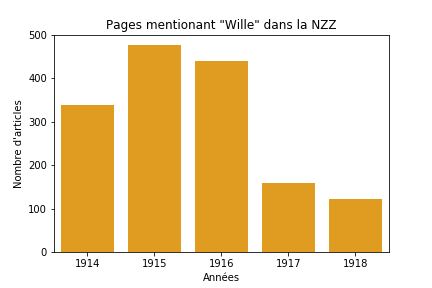
\includegraphics[width=8cm]{imgs/Wille_NZZ.png}
    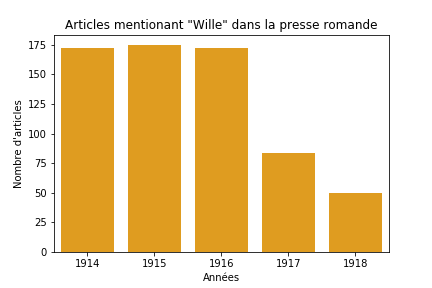
\includegraphics[width=8cm]{imgs/Wille_romands.png}
    \caption{Médiatisation du général Wille dans la NZZ et les journaux romands}
    \centering
    \label{fig:wille}
\end{figure}

Les articles mentionnant le général Wille entre juin et septembre 1914, c'est à dire au début de son mandat, sont dans les deux presses très peu critiques envers lui. 
Son élection n'est cependant pas vu de la même façon dans les deux zones linguistiques (figure \ref{fig:wille14}).
La presse romande voit cette élection comme obligatoire (\textit{nécessaire}). 
La presse alémanique dresse quant à elle un portrait élogieux du nouveau général, n'étant pas avare d'éloges (\textit{religiös}, \textit{menschlich}, \textit{modern}...).

Du côté romand, des articles critiquant le général apparaissent quelques mois après son élection et ce pendant tout son mandat.
Comme observable sur la figure \ref{fig:wille14-18}, il est souvent rappelé les affaires (\textit{accusation}, \textit{renseignement}, \textit{procédure}, \textit{jugement}) et les affinités (\textit{Bismarck}, \textit{Allemagne}) de Wille.
Du côté germanique, ces classes ne sont pas présentes, elles se limitent à un rôle plus descriptif de son rôle de général. Nous retrouvons donc des thèmes liès à la guerre, aux troupes et à l'administration fédérale.

\begin{figure}[h!]
    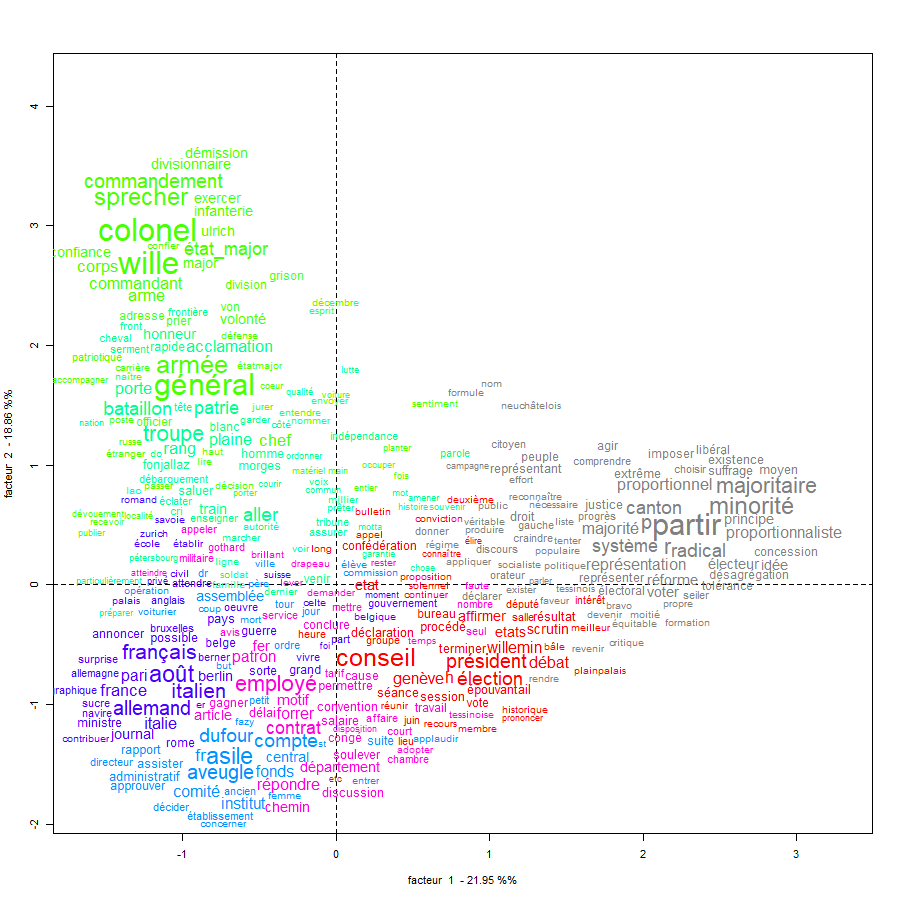
\includegraphics[width=8cm]{imgs/FR/Wille_15classes_election.png}
    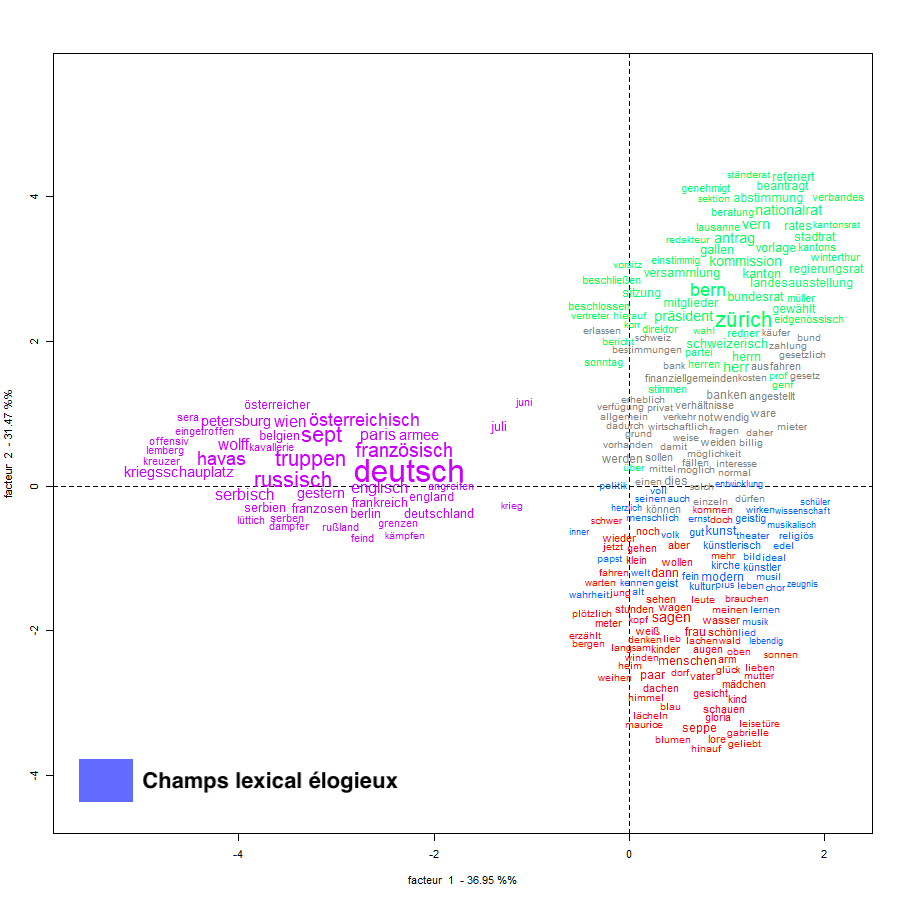
\includegraphics[width=8cm]{imgs/DE/Wille_15classes_election.png}
    \caption{Comparaison des classes de mots des articles francophones (diagramme de gauche) et germanophones (diagramme de droite) reliés au général Wille entre le 1\ier{} juin et le 30 septembre 1914.}
    \centering
    \label{fig:wille14}
\end{figure}

\begin{figure}[h]
    \centering
    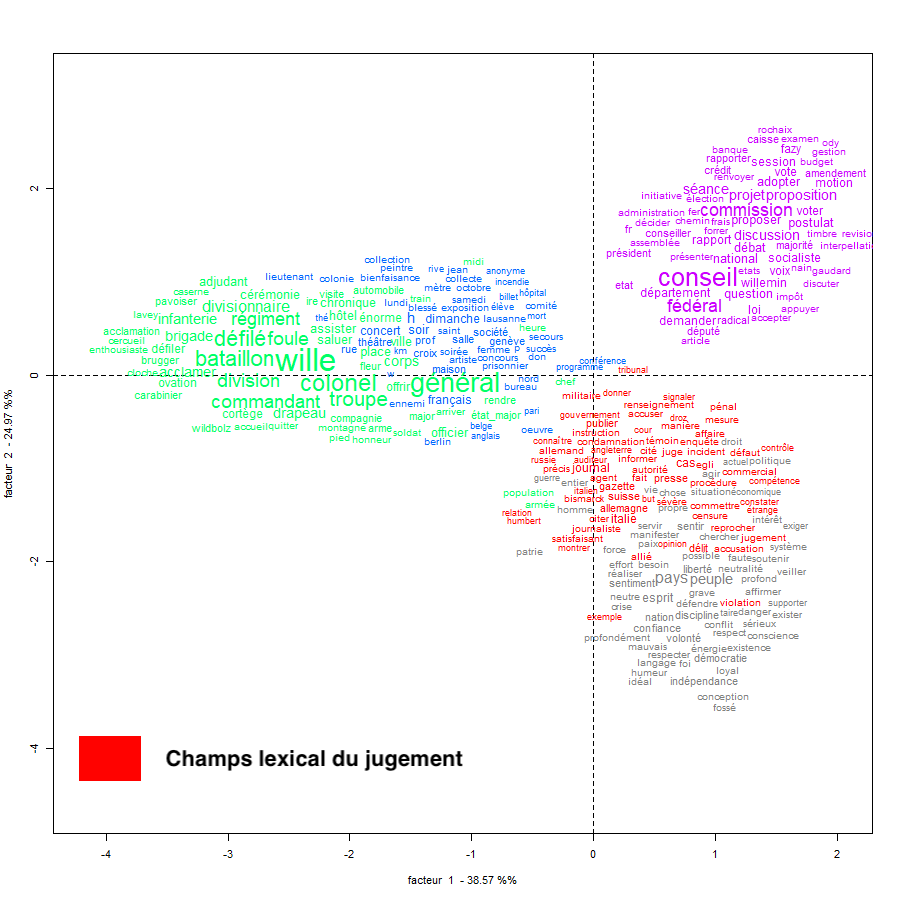
\includegraphics[width=12cm]{imgs/FR/Wille_10classes_mandat.png}
    \caption{Classes de mots des articles francophones reliés au général Wille entre le 1\ier{} octobre 1914 et le 31 décembre 1918.}
    \label{fig:wille14-18}
\end{figure}

\subsection*{Invasion de la Belgique}

Les points de vue entre les deux presses diffèrent aussi pour l'invasion de la Belgique.
Du côté alémanique, l'ultimatum est mentionné sans aucun autre qualificatif, alors que du côté romand (voir figure \ref{fig:belgique}) des questions se posent (\textit{indignation}, \textit{courage}, \textit{danger}, \textit{sacrifier}); la presse est plus critique.

\begin{figure}[h]
    \centering
    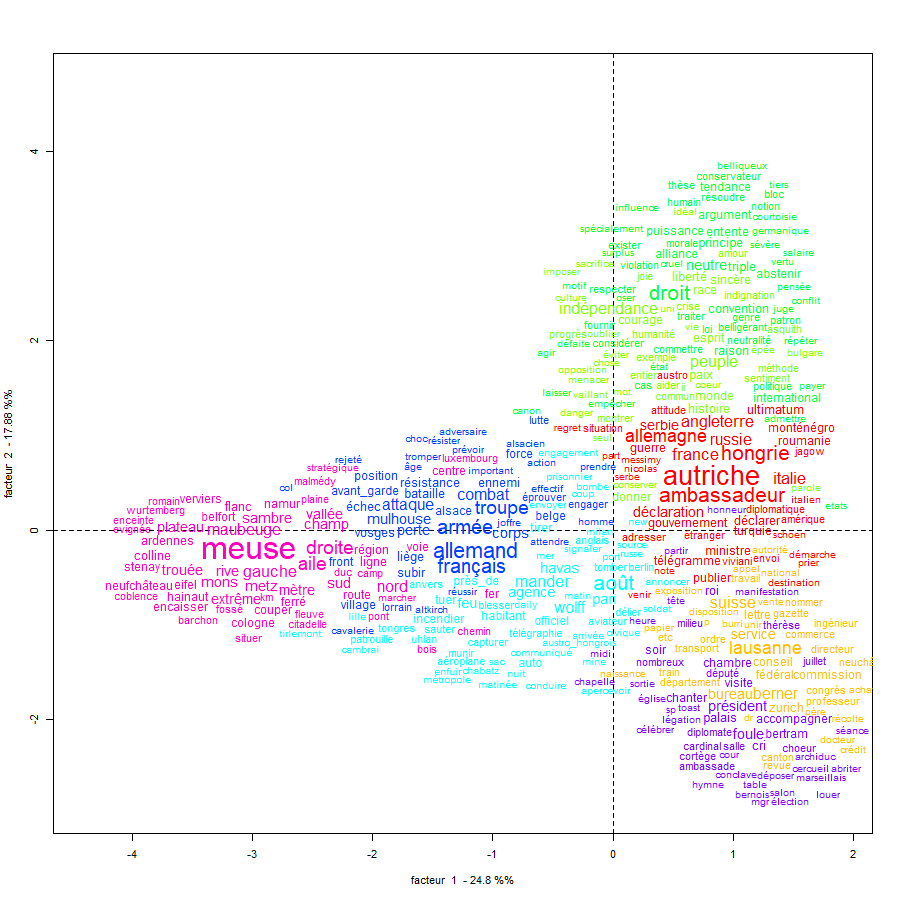
\includegraphics[width=12cm]{imgs/FR/Belgique_15classes.png}
    \caption{Classes de mots des articles francophones reliés à l'invasion de la Belgique entre le 1\ier{} juillet et le 1\ier{} septembre 1914.}
    \label{fig:belgique}
\end{figure}

\subsection*{L'affaire des colonels}

La presse romande relaie pleinement l'information alors que la presse alémanique semble l'ignorer.
Lors de notre analyse, une classe de mots parlant de l'affaire des colonels se démarque du côté francophone.
En effet, des mots tels que  \textit{affaire}, \textit{colonel}, \textit{Egli}, \textit{Wattenwyl}, \textit{enquête}, \textit{procès}  et \textit{espionnage} apparaissent dans la même classe de mots (voir figure \ref{fig:colonel}).
De plus, lors de l'analyse -- indépendante -- du mot-clé \textit{Wille} sur l'année 1916, l'affaire ressort aussi clairement au sein de sa propre classe de mots.
Ceci indique clairement la prévalence de l'affaire dans la presse romande, vu qu'ici notre recherche n'était pas concentrée sur celle-ci.

En revanche, du côté alémanique, absolument aucune classe de mot ne ressort avec ces mots-clés, traduisant une certaine volonté de la presse de réduire l'impact de l'affaire.

\begin{figure}[h!]
    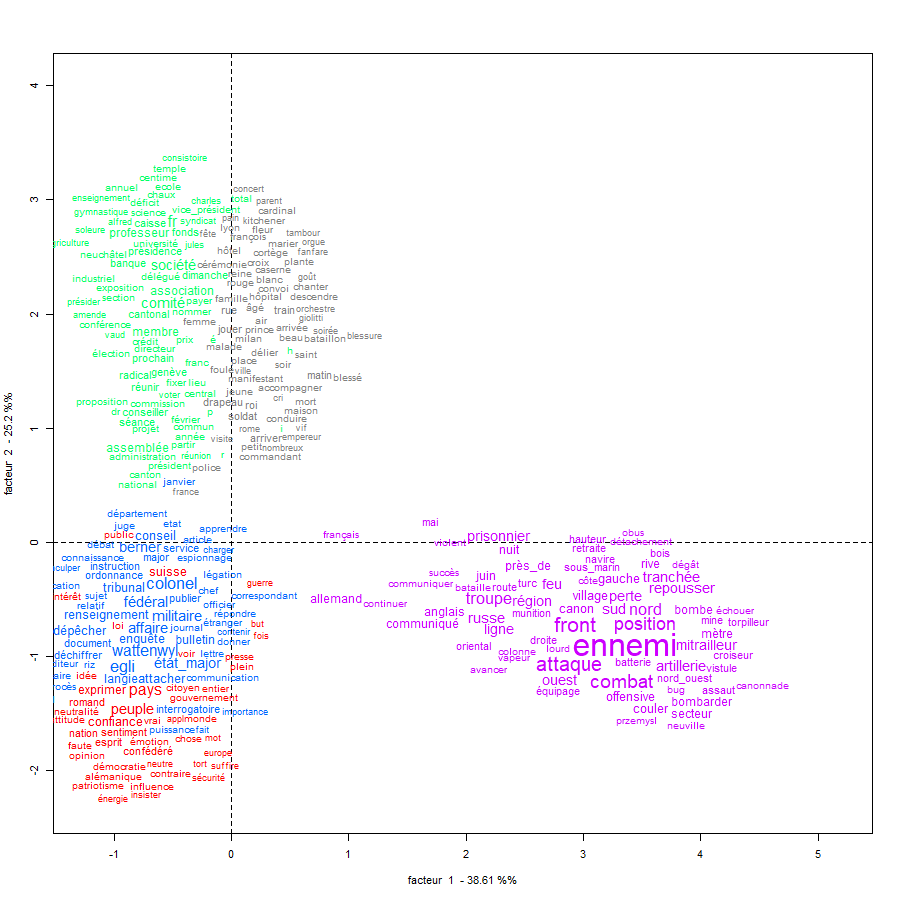
\includegraphics[width=8cm]{imgs/FR/affaire_colonel_10classes.png}
    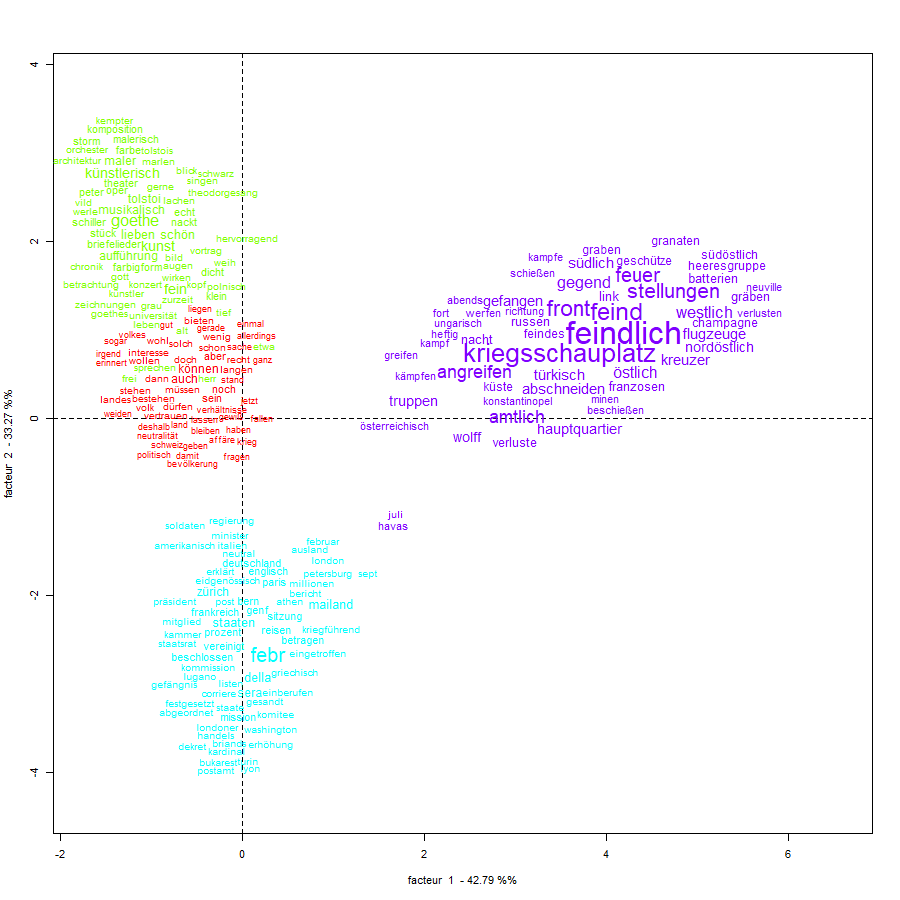
\includegraphics[width=8cm]{imgs/DE/Oberst10classes.png}
    \caption{Comparaison des classes de mots des articles francophones (diagramme de gauche) et germanophones (diagramme de droite) pour l'affaire des colonels.}
    \centering
    \label{fig:colonel}
\end{figure}

%classe bleue
%La classe jaune nous montre que les romands parlent beaucoup du jugement de cette affaire.

\subsection*{L'affaire Grimm-Hoffmann}

L'affaire est bien mentionnée des deux côtés de la Sarine et est couverte de manière similaire.
Une particularité les différencie cependant.
\textit{Grimm} est bien plus mentionné que \textit{Hoffmann} du côté francophone, alors que l'inverse est vrai du côté germanophone (voir figure \ref{fig:hoffmann}).
Cependant, du côté alémanique, le nom d'Hoffmann semble plus lié à son rôle gouvernemental (\textit{Präsident}, \textit{Bundesrat}) et à sa succession (\textit{Ador}) qu'à l'affaire en elle-même, où seul Grimm est présent.

\begin{figure}[h!]
    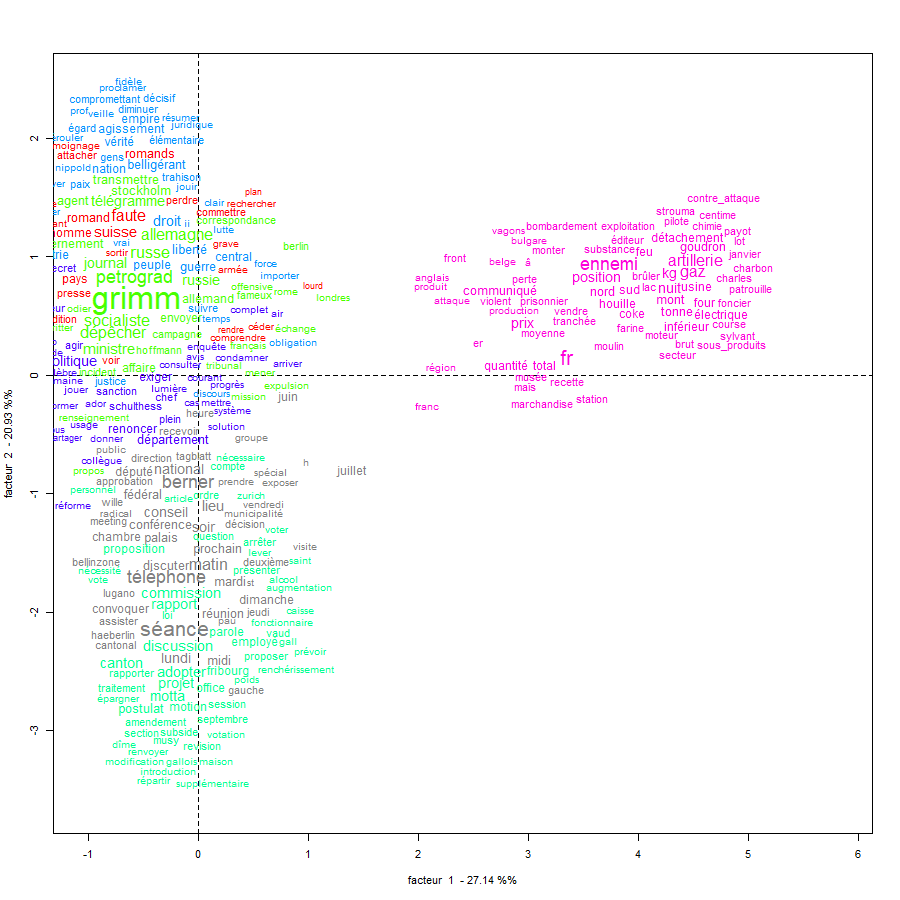
\includegraphics[width=8cm]{imgs/FR/Hoffmann_15classes.png}
    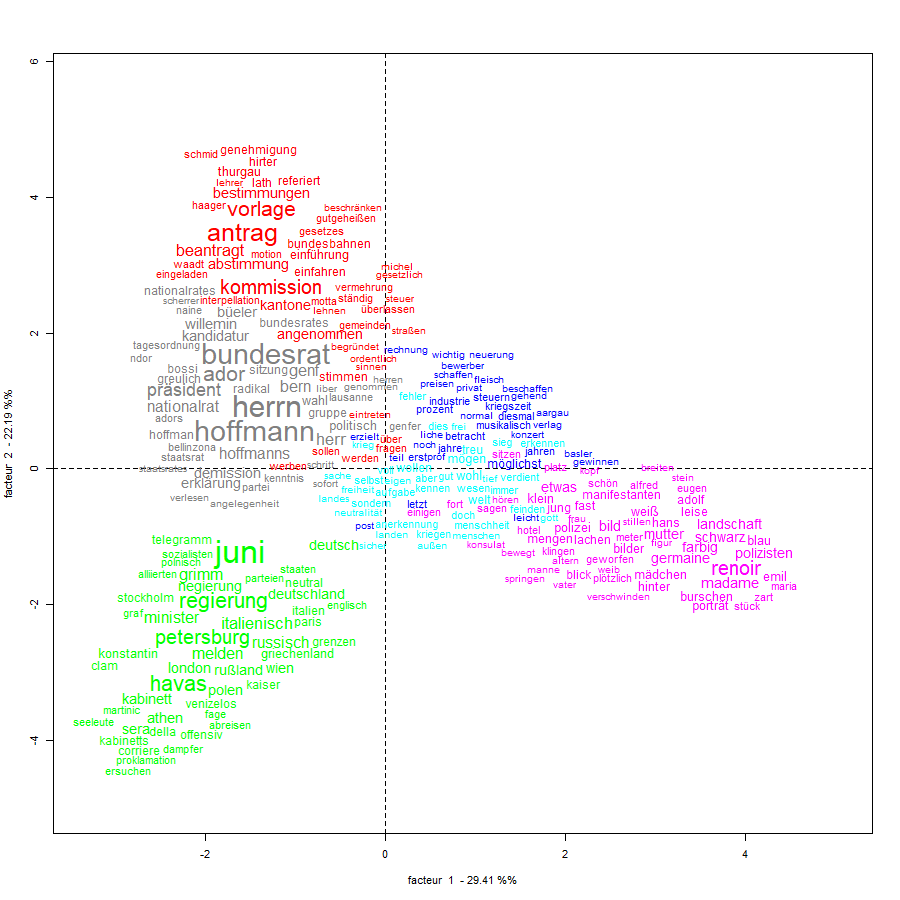
\includegraphics[width=8cm]{imgs/DE/Hoffmann_15classes.png}
    \caption{Comparaison des classes de mots des articles francophones (diagramme de gauche) et germanophones (diagramme de droite) pour l'affaire Grimm-Hoffmann.}
    \centering
    \label{fig:hoffmann}
\end{figure}

\subsection*{La grève générale}

Du côté de la presse romande nous voyons assez clairement que les articles liés à la grève générale de 1918 parlent du communisme et de la Russie.
Les mots \textit{bolchevisme}, \textit{Russie}, \textit{Lénine} apparaissent de nombreuses fois aux côtés de \textit{complot}, \textit{agitateur}, \textit{indépendance}, \textit{intérêt}.

\begin{figure}[ht!]
    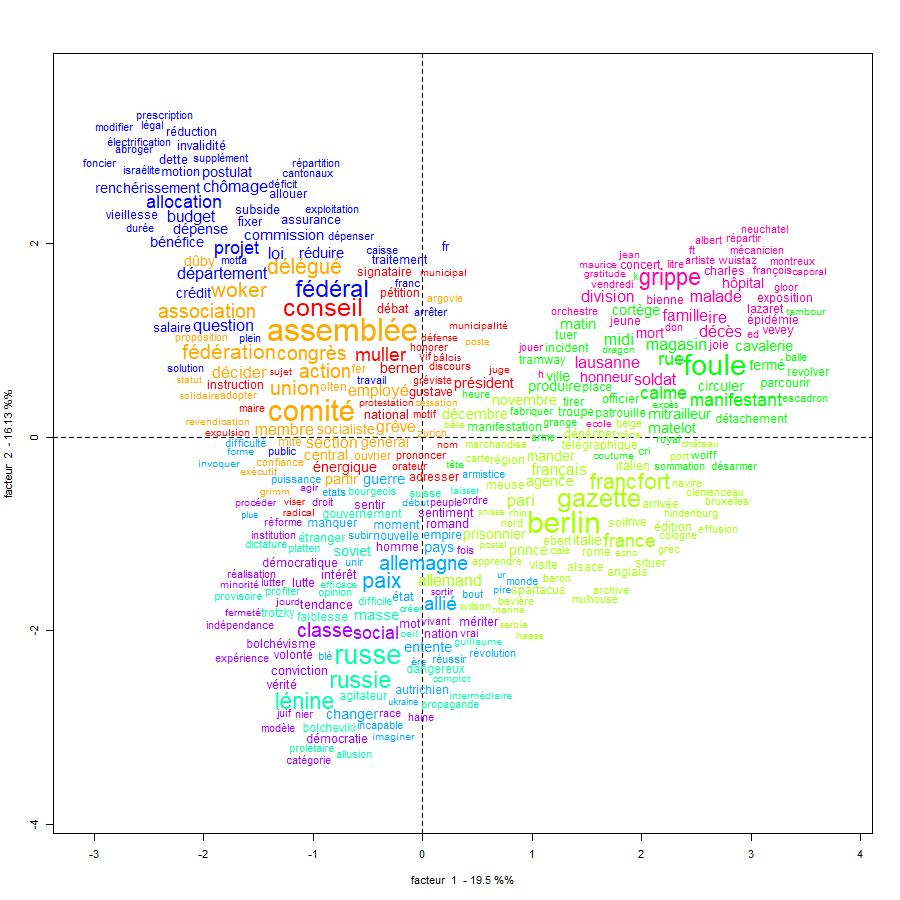
\includegraphics[width=8cm]{imgs/FR/greve_15classes.png}
    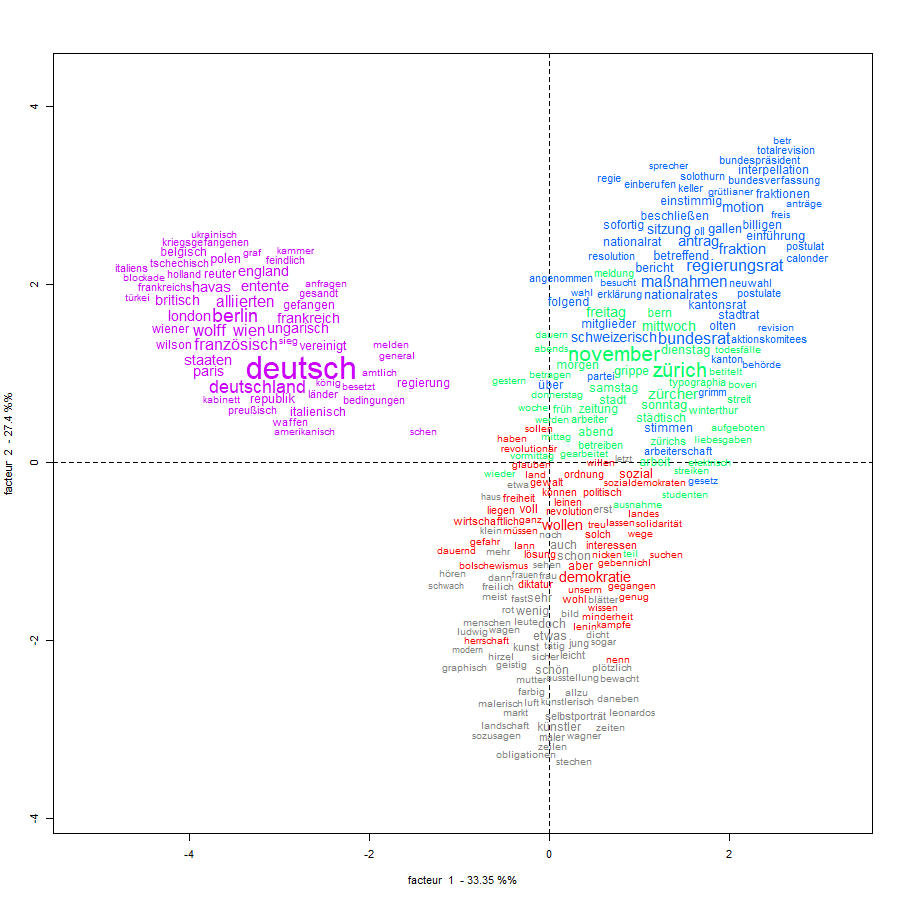
\includegraphics[width=8cm]{imgs/DE/Streik_15classes.png}
    \caption{Comparaison des classes de mots des articles francophones (diagramme de gauche) et germanophones (diagramme de droite) pour la grève générale.}
    \centering
    \label{fig:hoffmann2}
\end{figure}

La NZZ s'attarde moins sur la Russie.
Bien que le thème de la Russie est aussi abordé sur les mêmes pages que la grève, cela ne nous permet pas de faire un lien avec la grève générale de façon certaine.
Par contre, nous pouvons affirmer dans tous les cas que ce thème est moins important dans la NZZ.

Il nous paraît légitime de poser la question si les journaux romands analysés sont plus enclins à dénoncer cette grève en utilisant des liens soviétiques. 

\section*{Conclusion}

Les analyses textuelles d'Iramuteq nous ont permis d'identifier les regards divergeants des deux principales presses suisses au cours de la Première Guerre mondiale.
Nous avons pu remarquer que, de part sa proximité culturelle avec les pays de la Triple-Alliance, la presse alémanique avait tendance à cacher les principales affaires d'états liés aux pays germanophones (colonels et Grimm-Hoffmann).
La presse romande, quant à elle, semble, dans les analyses que nous avons pu faire, plus neutre et nuancée quand il s'agit d'évoquer les moments clefs de la guerre (invasion de la Belgique).

Dans un pays multiculturel comme la Suisse, des divergences d'opinion sont inévitables.
Les évènements que nous avons traités étaient les plus clivants, et c'est ce qui les rendaient intéressants à étudier.

Cependant, les résultats des analyses textuelles de la NZZ, de part les problèmes d'OCR ne sont pas autant exploitables que ceux de la presse romande et ainsi certaines classes de mots ont pu nous échapper.

\begin{thebibliography}{9}

\subsection*{Sources}

\bibitem{krieg}
\bsc{Freymond}, Jacques et al. (ed.).
Documents Diplomatiques Suisses, vol. 6, doc. 137: \og Le Général U. Wille au Chef du Département politique, A. Hoffmann \fg{} (20 juillet 1915).
Berne, 1981. Repéré à \url{https://dodis.ch/43412}

\bibitem{massacre}
Auteur inconnu.
Au jour le jour. \textit{Gazette de Lausanne}, p. 1.
Lausanne, 21 Novembre 1914.

\bibitem{apaisement}
\bsc{Freymond}, Jacques et al. (ed.).
Documents Diplomatiques Suisses, vol. 6, doc. 54: \og Aufruf an das Schweizervolk \fg{} (1\ier{} octobre 1914).
Berne, 1981.
Repéré à \url{https://dodis.ch/43329}

\bibitem{standpunkt} 
\bsc{Spitteler}, Carl.
\textit{Unser Schweizer Standpunkt}.
Zurich, 14 décembre 1914.

\bibitem{whistle_blower}
\bsc{Freymond}, Jacques et al. (ed.).
Documents Diplomatiques Suisses, vol. 6, doc. 160: \og A. Langie, cryptographe auprès de l’Etat-Major Général de l’Armée suisse au Chef du Département militaire, C. Decoppet \fg{} (8 décembre 1915).
Berne, 1981. Repéré à \url{https://dodis.ch/43435}

\bibitem{verdict}
Auteur inconnu.
Après le verdict. \textit{Gazette de Lausanne}, p. 5.
Lausanne, 1\ier{} mars 1916.

\bibitem{exclusion}
\bsc{Freymond}, Jacques et al. (ed.).
Documents Diplomatiques Suisses, vol. 6, doc. 214: \og Lettre collective des Cantons romands concernant les négociations avec l’Allemagne \fg{} (5 octobre 1916).
Berne, 1981. Repéré à \url{https://dodis.ch/43489}

\subsection*{Littérature secondaire}

\bibitem{division} 
\bsc{du Bois}, Pierre.
\textit{Union et division des Suisses. Les relations entre Alémaniques, Romands et Tessinois au XIXe et au XXe siècle}.
Lausanne, 1983.

\bibitem{place} 
\bsc{Elsig}, Alexandre.
\textit{Un ”laboratoire de choix”? La place de la Suisse dans le dispositif européen de la propagande allemande (1914-1918)}. 
Histoire de la Suisse et des Suisses, Editions Payot, 1982.

\bibitem{hoffmann}
\bsc{Stauffer}, Paul.
\textit{Die Affäre Hoffmann-Grimm}.
Schweizer Monatshefte, p. 1-30, 1973-1974.

\bibitem{clavien} 
\bsc{Clavien}, Alain.
\textit{Grandeurs et misères de la presse politique}.
Editions Antipodes, 2010.

\bibitem{delire} 
\bsc{Meienberg}, Nicolas.
\textit{Le Délire général. L’armée suisse sous influence}.
\bsc{Piccard}, Monique (trad.)
Edition Zoe, 1988 [1987].

\bibitem{grande_guerre}
\bsc{Rossfeld}, Roman \textit{et alii}.
\textit{14/18 La Suisse et la Grande Guerre}.
Editions Verlag Hier+Jetzt, 2014.

\bibitem{HistoireJost} 
\bsc{Jost}, Hans Ulrich.
\textit{Menace et Repliement}. 
Histoire de la Suisse et des Suisses, Editions Payot, 1982.
 
\bibitem{HistoireWalter} 
\bsc{Walter}, François.
\textit{Histoire de la Suisse. La création de la Suisse moderne (1830-1930)}.
Neuchâtel, Alphil-Presses universitaires suisses, 2013.

\bibitem{ilot} 
\bsc{Brand Crémieux}, Marie-Noëlle.
\textit{1914-1918 : la Suisse, un îlot dans la tourmente ?}.
Université Nice, 2017.

\subsection*{Médias}

\bibitem{wahl}
\bsc{Sprecher}, Daniel.
Intrigen, Verzögerungen und ein abendlicher Canossagang. \textit{Neue Zürcher Zeitung}.
Zurich, 2 août 2014.
Repéré à \url{https://www.nzz.ch/schweiz/intrigen-verzoegerungen-und-ein-abendlicher-canossagang-1.18355089}

\bibitem{propagande}
\bsc{Stephens}, Thomas.
Une Suisse inondée de propagande.
\textit{Swissinfo}. Berne, 2 septembre 2014.
\url{https://www.swissinfo.ch/fre/culture/premi\%C3\%A8re-guerre-mondiale_une-suisse-inond\%C3\%A9e-de-propagande/40585506}

\bibitem{rede_spitteler}
\bsc{Münger}, Felix.
Die Rede, für die Carl Spitteler bitter bezahlen musste. \textit{Schweizer Radio und Fernsehen}.
Zurich, 4 avril 2019.
Repéré à \url{https://www.srf.ch/kultur/literatur/unser-schweizer-standpunkt-die-rede-fuer-die-carl-spitteler-bitter-bezahlen-musste}

\bibitem{sprachenfrieden}
\bsc{Büchi}, Christophe.
Der holprige Weg zum schweizerischen Sprachenfrieden. \textit{Neue Zürcher Zeitung}.
Zurich, 18 novembre 2018.
Repéré à \url{https://www.nzz.ch/schweiz/der-holprige-weg-zum-schweizerischen-sprachenfrieden-ld.1437249}

\subsection*{Technique}

\bibitem{dict-de}
\bsc{Naber}, Daniel.
German part-of-speech dictionary. \textit{LanguageTool.org}.
CC-BY-SA-4.0. 2019.
Disponible sur \url{https://github.com/languagetool-org/german-pos-dict}

\end{thebibliography}

\end{document}
